\input templates/header
\title[ASD - Introduzione]{\textbf{Algoritmi e Strutture Dati}\\[24pt]Introduzione}

\graphicspath{{figs/A2/}}

\title[ASD - Algoritmo di Tarjan]{\textbf{Algoritmi e strutture dati}\\[24pt]Algoritmo di Tarjan per\\Strongly Connected Components}

\begin{document}

%-------------------------------------------------------------------------
\FrameTitle{}

%-------------------------------------------------------------------------
\FrameContent


%%%%%%%%%%%%%%%%%%%%%%%%%%%%%%%%%%%%%%%%%%%%%%%%%%%%%%%%%%%%%%%%%%%%%%%%%%
\section{Descrizione algoritmo}

\newcommand{\Index}{\mathit{index}}
\newcommand{\LowLink}{\mathit{lowlink}}
\newcommand{\Current}{\mathit{current}}
\newcommand{\inStack}{\mathit{inStack}}


\begin{frame}{Algoritmo}

\begin{Procedure}
\caption[A]{\Set\ \scc(\Graph $G$)} 
$\INTEGER\ \Current \gets 1$\;
$\INTARRAY\ \Index \gets \NEW\ \INTEGER[1 \ldots G.n] \gets \{ 0, \ldots, 0 \}$\;
$\INTARRAY\ \LowLink \gets \NEW\ \INTEGER[1 \ldots G.n]$\;
$\BOOLEAN[\,]\ \inStack \gets \NEW\ \BOOLEAN[1 \ldots G.n]$\;
$\Stack\ \mathit{stack} \gets \stackconstructor()$\;
$\Set\ \mathit{components} \gets \setconstructor()$\;
\ForEach{$u \in G.\VV()$}{
  \If{$\Index[u] = 0$}{
    $\textsf{strongconnect}(G, u)$\;
  }
}
\end{Procedure}

\end{frame}

\begin{frame}[shrink]{Algoritmo}

\begin{Procedure}
\caption[A]{$\textsf{strongconnect}(\Graph\ g, \Node\ u)$}
$\Index[u] \gets \LowLink[u] \gets \Current$\;
$\Current \gets \Current+1$\;
$\mathit{stack}.\stackpush(u)$\;
$\inStack[u] \gets \TRUE$\;
\ForEach{$v \in G.\adj(u)$}{
  \uIf{$\Index[v] = 0$}{
    $\textsf{strongconnect}(G, v)$\;
	$\LowLink[u] = \MIN(\LowLink[u], \LowLink[v])$\;
  }\ElseIf{$\inStack[v]$}{
	$\LowLink[u] = \MIN(\LowLink[u], \LowLink[v])$\;
  }
}

\If{$\LowLink[u] = \Index[u]$}{
  $\Set\ \mathit{component} \gets \setconstructor()$\; 
  \Repeat{$w=u$}{
  $\Node\ w \gets \mathit{stack}.\stackpop()$\;
  $\inStack[w] \gets \FALSE$\;
  $\mathit{component}.\setinsert(w)$\;
  }
  $\mathit{components}.\setinsert(\mathit{component})$\;
}
\end{Procedure}

\end{frame}

\begin{frame}{Esempio di funzionamento}
\begin{figure}
\begin{overprint}
\onslide<1|handout:1>\centering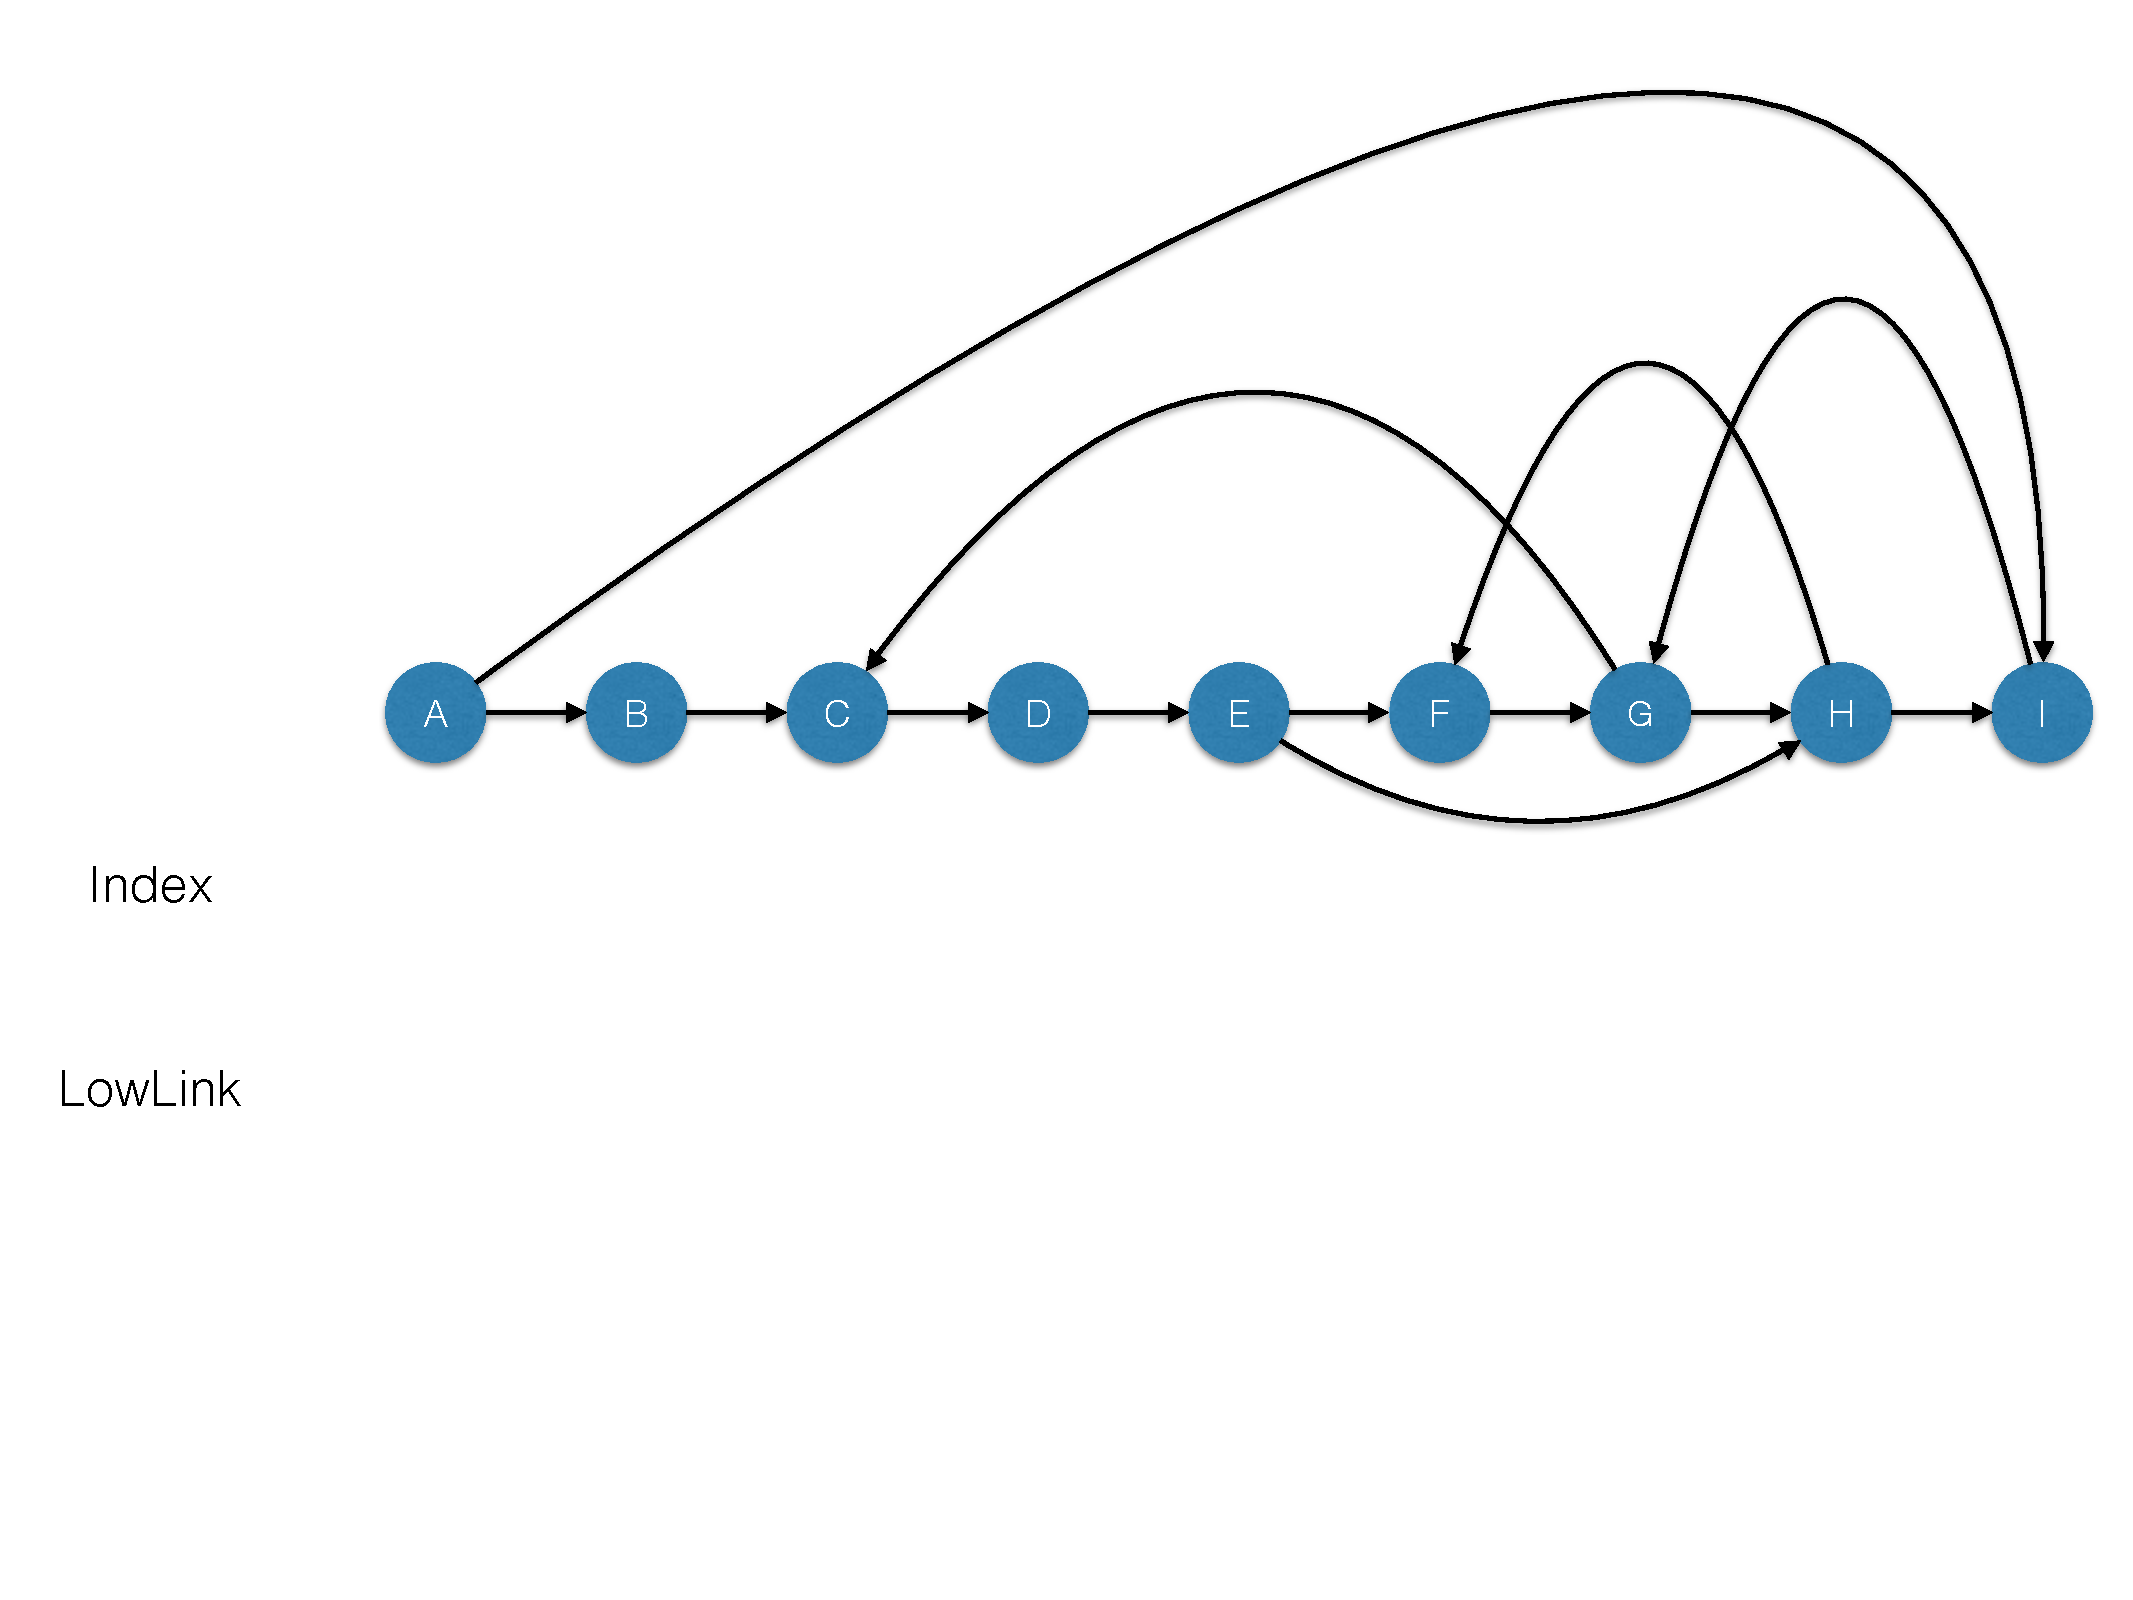
\includegraphics[width=11cm,page=1]{figura-tarjan.pdf}
\onslide<2|handout:2>\centering\includegraphics[width=11cm,page=2]{figura-tarjan.pdf}
\onslide<3|handout:3>\centering\includegraphics[width=11cm,page=3]{figura-tarjan.pdf}
\onslide<4|handout:4>\centering\includegraphics[width=11cm,page=4]{figura-tarjan.pdf}
\onslide<5|handout:5>\centering\includegraphics[width=11cm,page=5]{figura-tarjan.pdf}
\onslide<6|handout:6>\centering\includegraphics[width=11cm,page=6]{figura-tarjan.pdf}
\onslide<7|handout:7>\centering\includegraphics[width=11cm,page=7]{figura-tarjan.pdf}
\onslide<8|handout:8>\centering\includegraphics[width=11cm,page=8]{figura-tarjan.pdf}
\onslide<9|handout:9>\centering\includegraphics[width=11cm,page=9]{figura-tarjan.pdf}
\onslide<10|handout:10>\centering\includegraphics[width=11cm,page=10]{figura-tarjan.pdf}
\onslide<11|handout:11>\centering\includegraphics[width=11cm,page=11]{figura-tarjan.pdf}
\onslide<12|handout:12>\centering\includegraphics[width=11cm,page=12]{figura-tarjan.pdf}
\onslide<13|handout:13>\centering\includegraphics[width=11cm,page=13]{figura-tarjan.pdf}
\onslide<14|handout:14>\centering\includegraphics[width=11cm,page=14]{figura-tarjan.pdf}
\onslide<15|handout:15>\centering\includegraphics[width=11cm,page=15]{figura-tarjan.pdf}
\onslide<16|handout:16>\centering\includegraphics[width=11cm,page=16]{figura-tarjan.pdf}
\onslide<17|handout:17>\centering\includegraphics[width=11cm,page=17]{figura-tarjan.pdf}
\onslide<18|handout:18>\centering\includegraphics[width=11cm,page=18]{figura-tarjan.pdf}
\onslide<19|handout:19>\centering\includegraphics[width=11cm,page=19]{figura-tarjan.pdf}
\onslide<20|handout:20>\centering\includegraphics[width=11cm,page=20]{figura-tarjan.pdf}
\onslide<21|handout:21>\centering\includegraphics[width=11cm,page=21]{figura-tarjan.pdf}
\end{overprint}
\end{figure}
	
\end{frame}	


\end{document}





